\lab{Algorithms}{K-Means Clustering}{K-Means Clustering}
\objective{Understand the basics of k-means clustering}

Recall the iris dataset transformed under PCA, where we only kept the first two principal components.

\begin{figure}
\centering
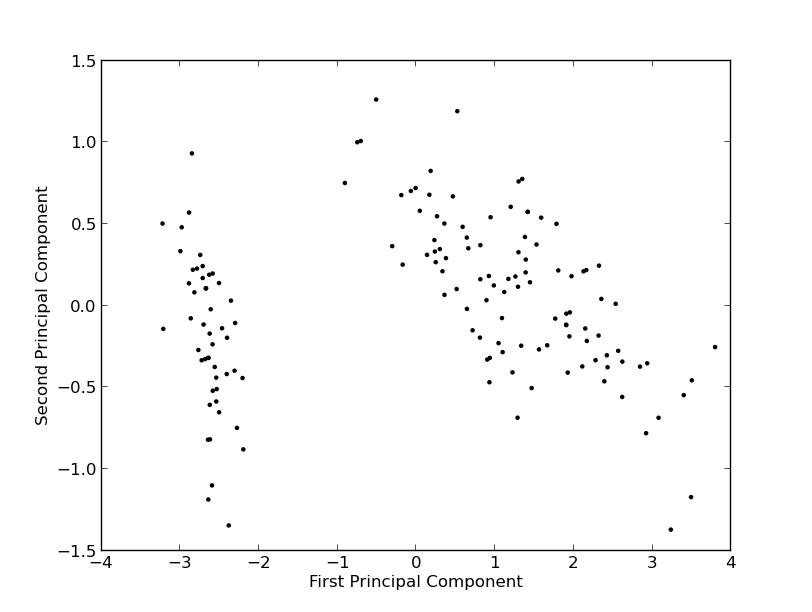
\includegraphics[width=\textwidth]{irispca.jpg}
\end{figure}

A human can easily see that there are two very distinct groups of irises, but how can we create an algorithm to do this without human supervision? This task is called \emph{unsupervised learning} or \emph{clustering}. The objective is to seek a partition of the data, where points in the same subset will be ``close'' according to some metric. The metric used will likely depend on the data, but some obvious ones include euclidean distance and angular distance. Throughout this lab we will use the metric $d(x,y)$, the euclidean distance between $x$ and $y$.

More formally, let 
\begin{equation*}
\mathbf{X} = \left( \mathbf{x_{1}}, \mathbf{x_{2}}, \cdots, \mathbf{\x_{n}}\right)
\end{equation*}
be a set of observations, each having $K$ features. We would like to partition $\mathbf{X}$ into $N$ \emph{clusters}
\begin{equation*}
\mathbf{S} = \left( S_{1}, S_{2}, \cdots, S_{N}\right)
\end{equation*}
such that for each $S_{i}$, the observations in $S_{i}$ are all ``close''. More formally, we would like to find the partition $\mathbf{S}$ such that the within-cluster sum of squares is minimized, i.e. 
\begin{equation*}
\mathbf{S^{*}} = \text{argmin}_{\mathbf{S}} \sum_{i=1}^{N} \sum_{\mathbf{x_{j}} \in S_{i}} \norm{\mathbf{x_{j}} - \mathbf{\mu_{i}}}
\end{equation*}
where $\mathbf{\mu_{i}}$ is the mean of the observations in $S_{i}$.

Finding this global minimizing partition $\mathbf{S}$ is generally intractable, but the \emph{k-means} algorithm is a heuristic approach that can often provide good results. K-means seems like a little brother to Gaussian Mixture Models, as it is a variation of the EM algorithm. We begin by specifying an initial cluster centroid $\mathbf{\mu_{i}}^{(1)}$ for each $i = 1, \cdots, N$.

\begin{figure}[h]
\centering
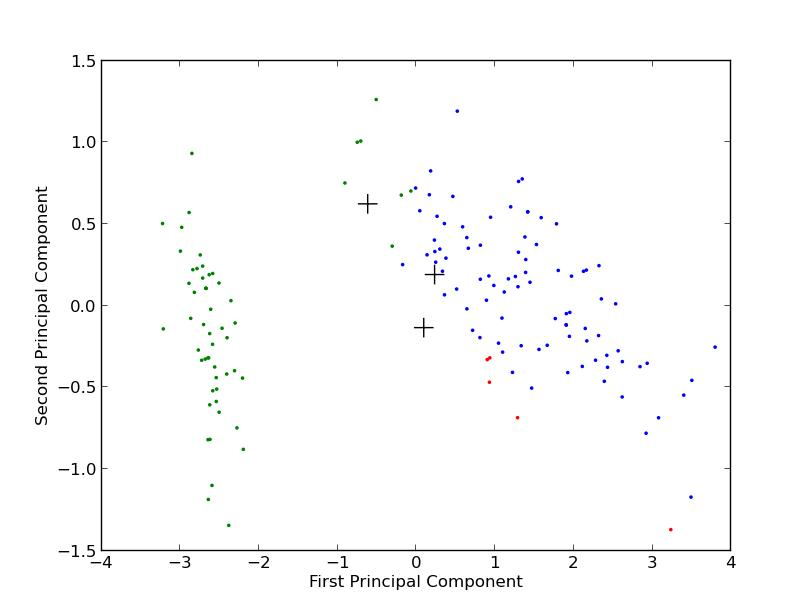
\includegraphics[width=\textwidth]{iteration1.jpg}
\caption{Clusters at iteration 1}
\end{figure}

For each iteration, we adopt the following procedure. Given a current set of cluster centroids $\mathbf{\mu}^{(t)}$, we find a partition $\mathbf{S}^{(t)}$ of the observations such that 
\begin{equation*}
S_{i}^{(t)} = \{\mathbf{x} \; : \; \norm{\mathbf{x} - \mathbf{\mu}_{i}^{(t)}} \leq \norm{\mathbf{x} - \mathbf{\mu}_{j}^{(t)}} \forall j = 1, \cdots, N\}
\end{equation*}
This is similar to the expectation step in EM for GMMs.

\begin{figure}[h]
\centering
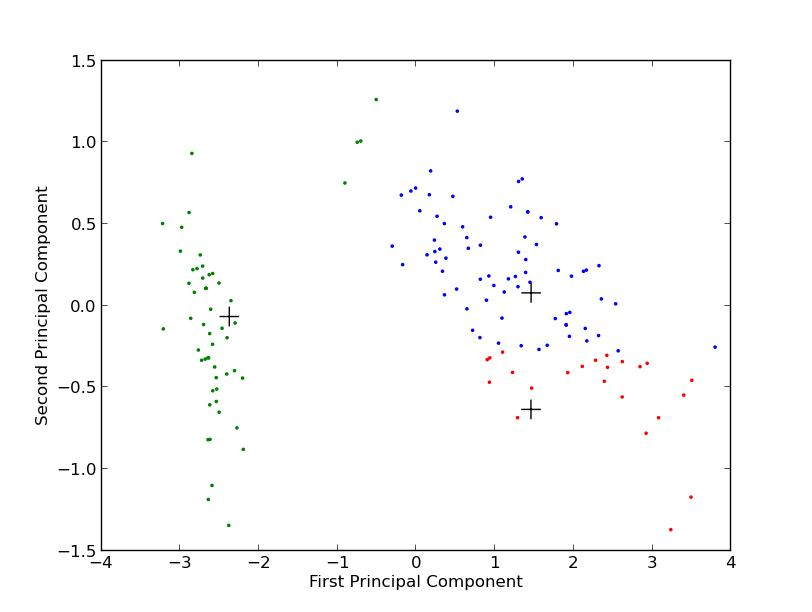
\includegraphics[width=\textwidth]{iteration2.jpg}
\caption{Clusters at iteration 2}
\end{figure}

We then update our cluster centroids by computing for each $i = 1, \cdots, N$,
\begin{equation*}
\mathbf{\mu}_{i}^{(t+1)} = \frac{\sum_{\mathbf{x} \in S_{i}^{(t)}} \mathbf{x}}{|S_{i}^{(t)}|}
\end{equation*}
This is similar to the maximization step in EM for GMMs.

We continue to iterate in this manner until the partition ceases to change. Between the fifth and sixth iteration, the partition stays the same, so the process has converged. If we look closely and compare this with our results from the PCA lab, we will see that this heuristic algorithm has nearly clustered the iris observations by species!

\begin{figure}[h]
	\centering
	\begin{tabular}{cc}
	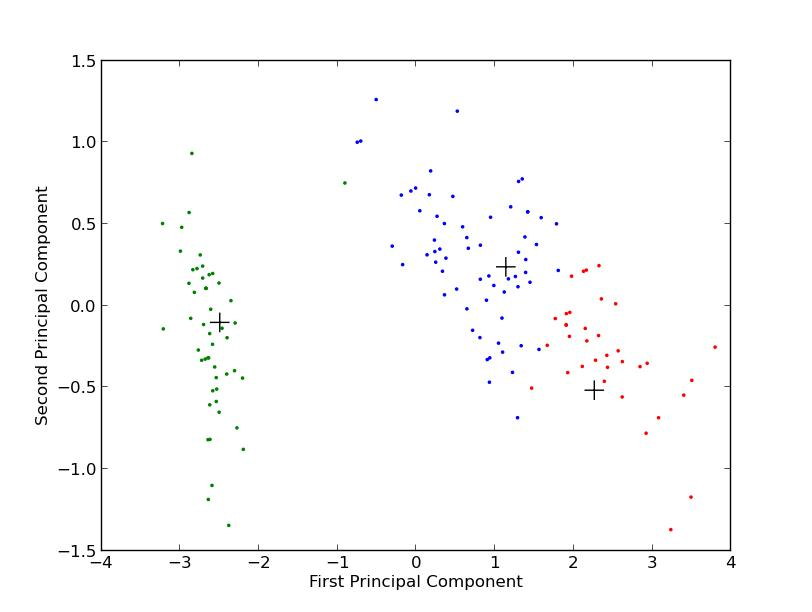
\includegraphics[width=.49\textwidth]{iteration3.jpg} & 
	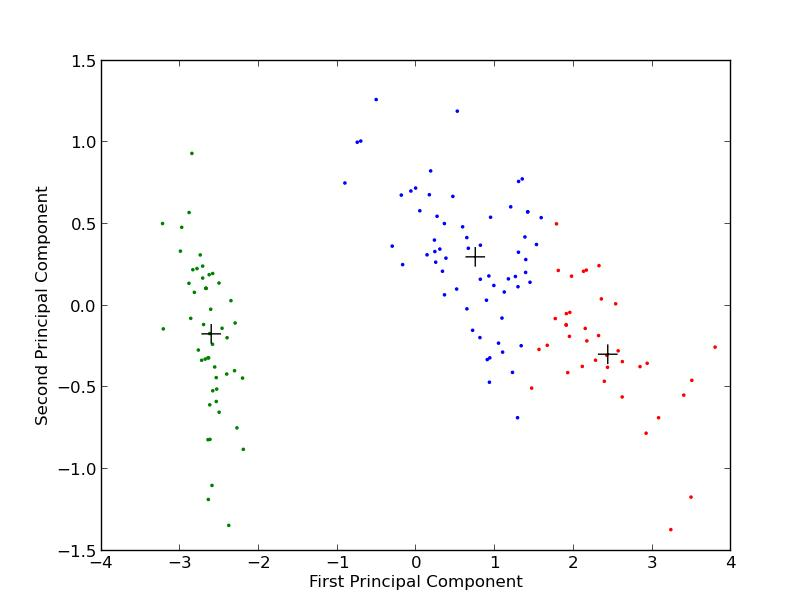
\includegraphics[width=.49\textwidth]{iteration4.jpg} \\
	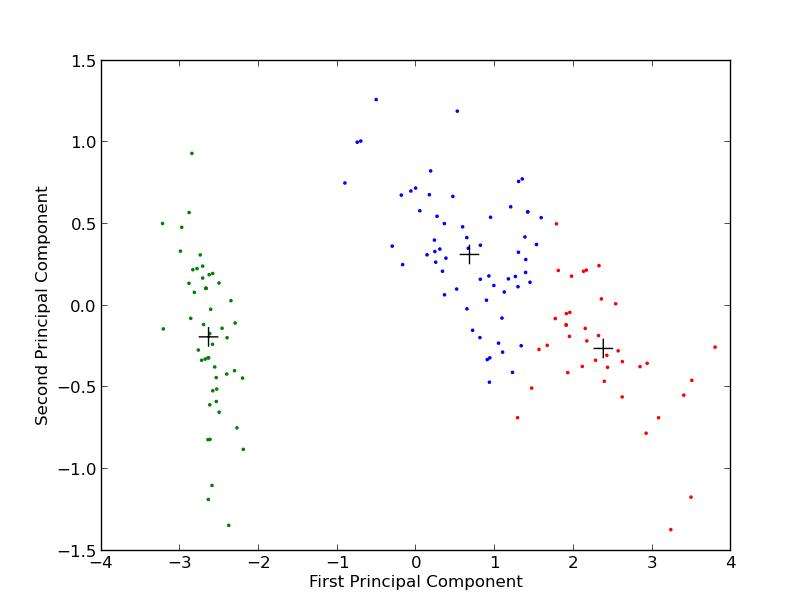
\includegraphics[width=.49\textwidth]{iteration5.jpg} & 
	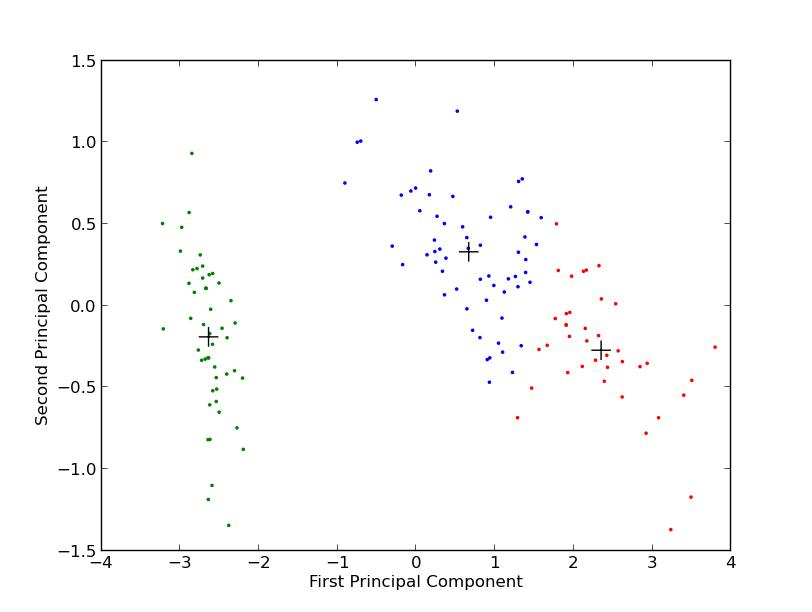
\includegraphics[width=.49\textwidth]{iteration6.jpg}
	\end{tabular}
	\caption{Clusters at iterations 3 through 6}
\end{figure}

\begin{problem}
Write a function that accepts the number of clusters $N$ and the number of features $K$, and returns a random initialization consisting of $N$ centroids, each of length $K$. How you randomly initialize is up to you, but it might be wise to include a parameter that allows you to change the variance of the distribution you are drawing from. This is important, because even though all of the transformed iris observations are near the origin, this will not always be the case, so we should be able to initialize both near the origin, and far from it. Also include a boolean parameter to determine whether or not the centroids should be normalized (this will be important for the next lab).
\end{problem}

\begin{problem}
Write a function that computes the euclidean distance between two vectors. Write a function that accepts a set of observations, your current set of centroids, and a distance function f, and returns the partition of observations described above. The return value can simply be an array where the $i^{th}$ entry denotes the cluster to which the $i^{th}$ observation has been assigned.
\end{problem}

\begin{problem}
Write a function that accepts a set of observations and their cluster assignments, and which updates the centroids. Add another boolean parameter to determine whether or not the centroids should be normalized. If a cluster is empty, do nothing to its centroid.
\end{problem}

\begin{problem}
Write a function to perform the k-means algorithm, using the functions made above.
\end{problem}

\begin{problem}
Write a function that accepts a set of observations, cluster assignments, and centroids, and plots each cluster as a different color, and then plots each centroid with a ``+'' mark. Test your k-means algorithm on the transformed iris data set several times, and plot each outcome.
\end{problem}
